\section{Geant4シミュレーションによるテスト実験の再現}
製作したコーン型ライトガイドの集光性能を確認するため、Geant4シミュレーションによるプロトタイプ検出器の再現を行った。
コーン型ライトガイドの集光性能を確認することで、実機のシミュレーションにおいてより正確なシミュレーションを行うことができる。

\subsection{ジオメトリ}

\begin{figure}[htbp]
  \centering
  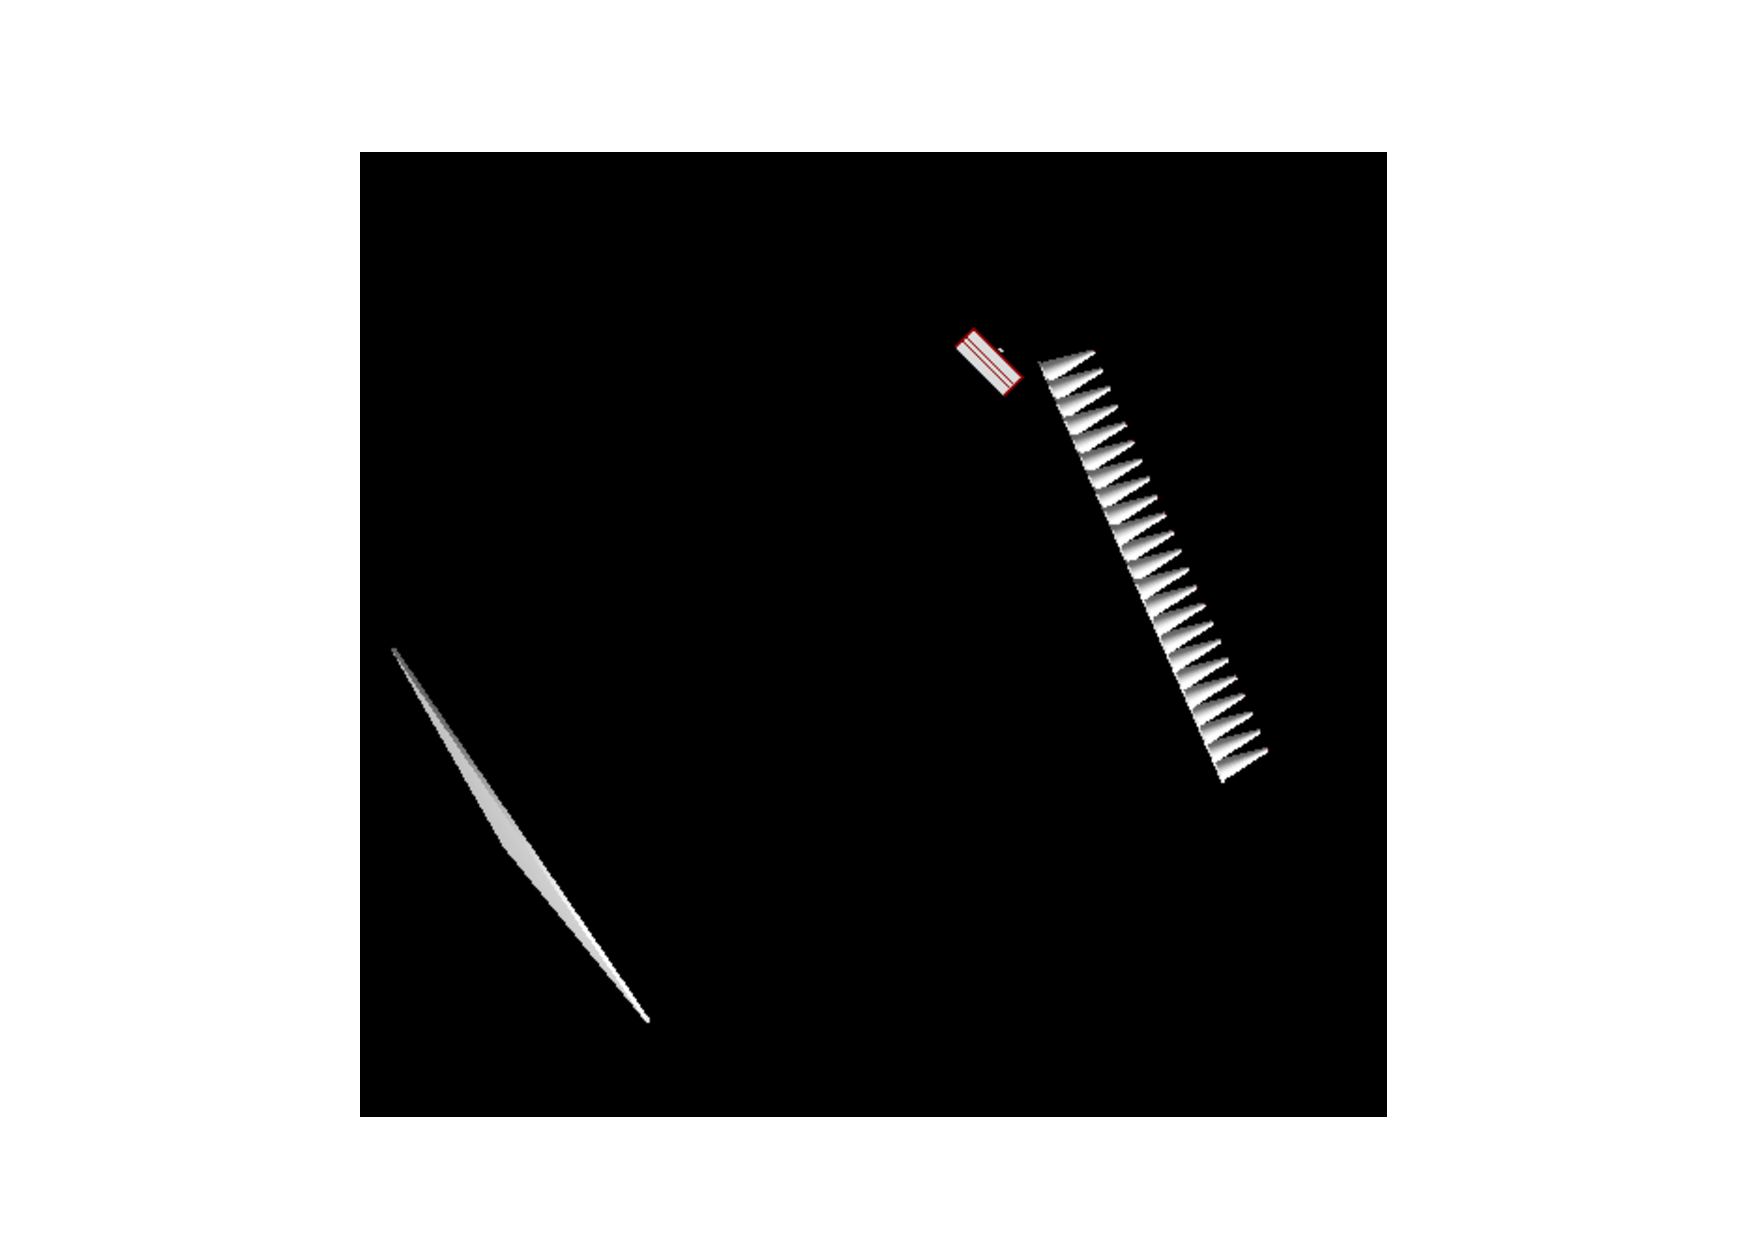
\includegraphics[width=10cm, page=1]{images/chapter4/ELPHsimulationSetup.pdf}
  \caption{テスト実験再現用シミュレーションのセットアップ。上から見た図。}
  \label{fig:ELPHsimulationSetup1}
\end{figure}

\subsection{エアロゲル}
エアロゲルはサイズ、屈折率、透過長、吸収長、をパラメータとして考慮した。
また、テスト実験で使用した3つのエアロゲルの個体差も考慮してパラメータの設定を行った。
表にシミュレーションで使用した各エアロゲルのパラメータを示す。
屈折率は波長に依らず一定とし、透過長はレイリー散乱の波長の4乗に比例する関係を考慮した。
吸収長は全てのエアロゲルで波長に依らず5500 mmとし、縦横のサイズは全て$\SI{146}{mm}\times\SI{146}{mm}$とした。
% \begin{table}[htbp]
%   \caption{使用したエアロゲルのパラメータ}
%   \label{table:Aerogel}
%   \centering
%   \begin{tabular}{cccc}
%     \hline
%     型番      & 屈折率    & 厚さ (mm) & 波長400 nmに対する透過長 (mm) \\
%     \hline\hline
%     TSA9-3  & 1.0400 & 20.7    & 54                   \\
%     TSA10-3 & 1.0395 & 10.8    & 55                   \\
%     TSA9-4  & 1.0397 & 21.0    & 58                   \\
%     \hline
%   \end{tabular}
% \end{table}

\subsection{球面鏡}
球面鏡は、曲率半径$2982 \si{mm}$、外径は$\SI{1009}{mm}\times\SI{1009}{mm}$とした。
反射率は、図を参考に波長依存性を考慮して設定した。




\subsection{MPPC}
MPPCは図を参考に、受光面を$\SI{6}{mm}(縦)\times\SI{6}{mm}(横)\times\SI{1.3}{mm}(厚さ)$のシリコンとし、
受光面の上に窓材として厚さ$\SI{4}{mm}$のシリコンを設定した。
受光面のシリコンは屈折率1.41、吸収長
\begin{figure}
  \centering
  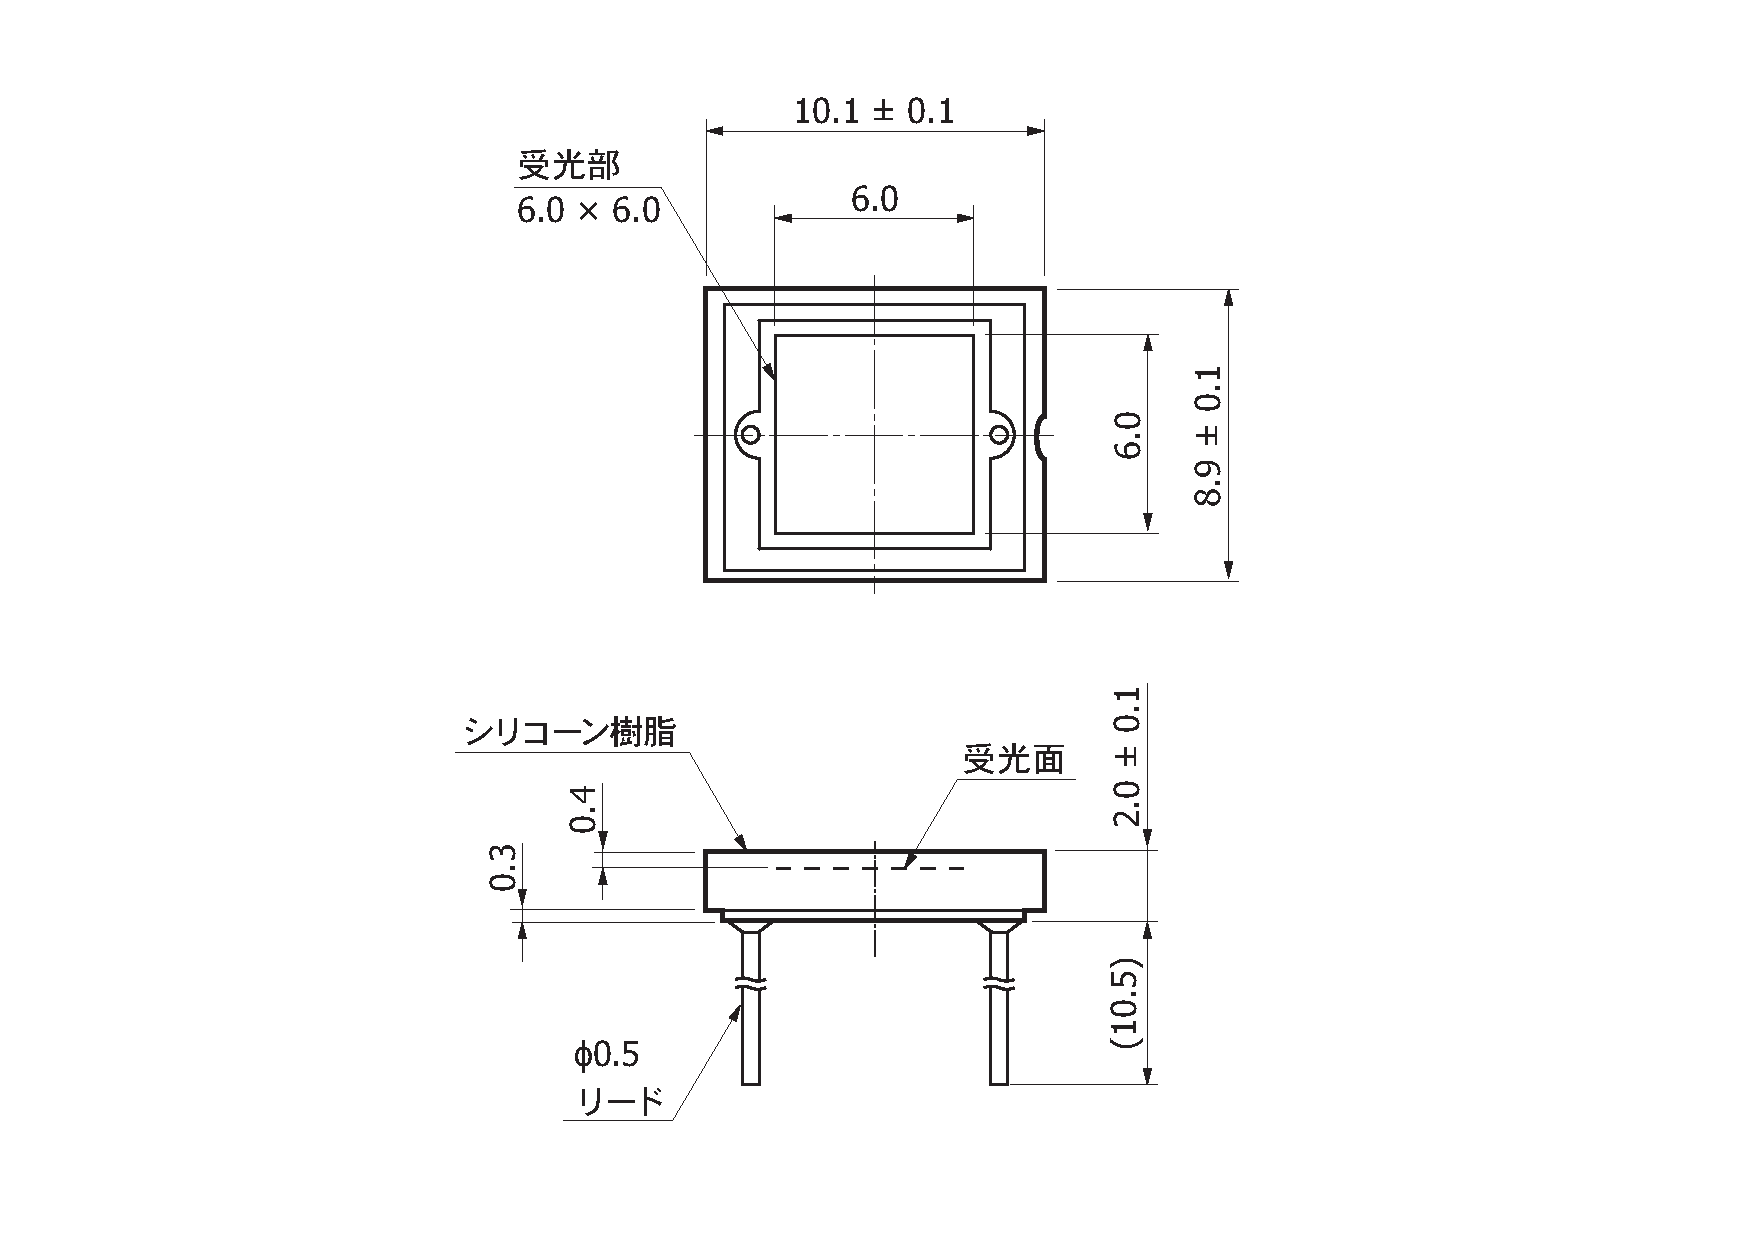
\includegraphics[width=15cm]{images/chapter4/MPPCshape.pdf}
  \caption{使用したMPPCの構造。。}
  \label{fig:MPPCshape}
\end{figure}

\subsection{コーン型ライトガイド}



\begin{figure}[htbp]
  \centering
  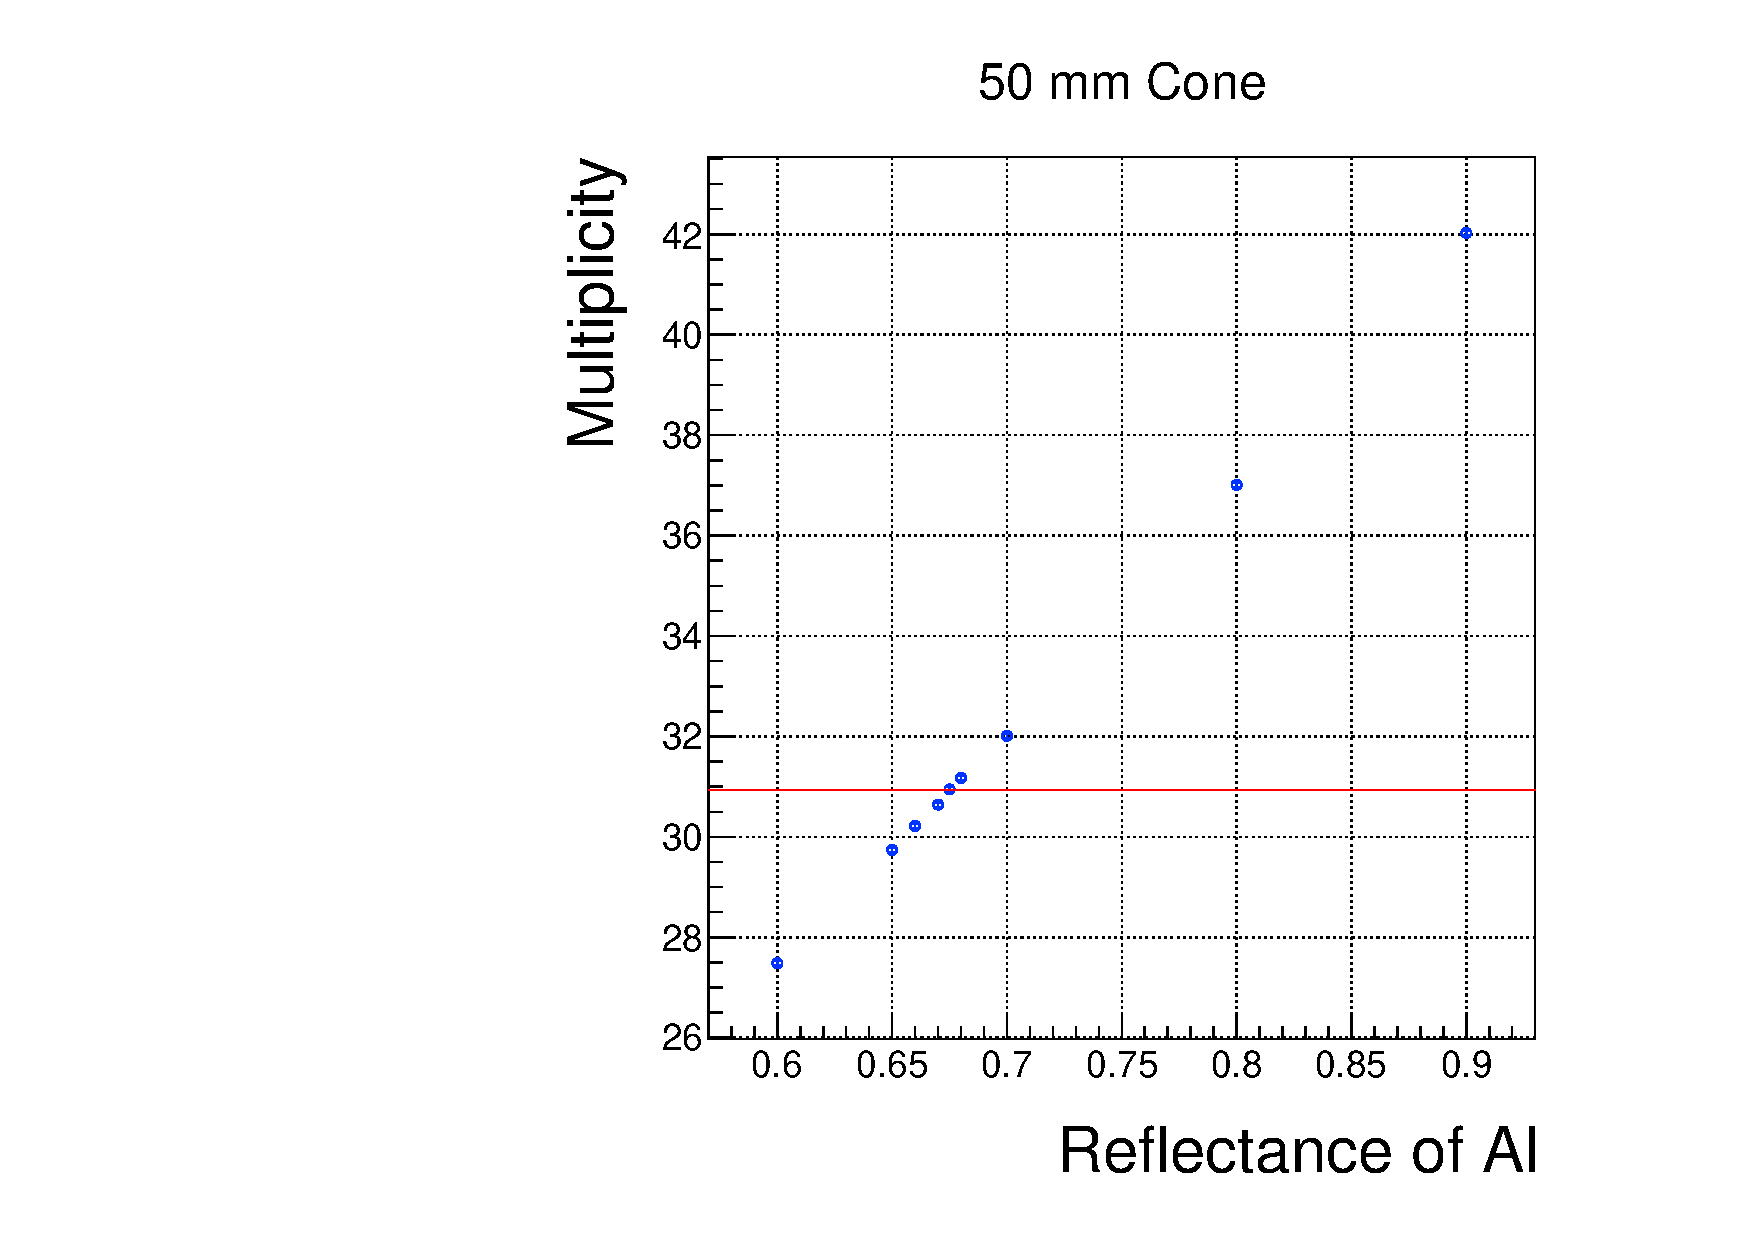
\includegraphics[width=10cm, page=1]{images/chapter4/decideAl.pdf}
  \caption{$\SI{50}{mm}$コーンの場合の、コーン反射面の反射率に対するMultiplicityの変化。赤のラインが実験値の値。反射率を0.675とすることで実験値を再現できる。}
  \label{fig:decideAl_50}
\end{figure}
\begin{figure}[htbp]
  \centering
  \includegraphics[width=10cm, page=2]{images/chapter4/decideAl.pdf}
  \caption{$\SI{30}{mm}$コーンの場合の、コーン反射面の反射率に対するMultiplicityの変化。赤のラインが実験値の値。反射率を0.67とすることで実験値を再現できる。}
  \label{fig:decideAl_30}
\end{figure}